%----------------------------------------------------------------------------------------
%
% LaTeX-template for degree projects at LNU, Department of Computer Science
% Last updated by Johan Hagelbäck, Oct 2015
% Linnaeus University
%
% License: Creative Commons BY
%
%----------------------------------------------------------------------------------------

%----------------------------------------------------------------------------------------
%	Settings and configuration
%----------------------------------------------------------------------------------------

\documentclass[a4paper,12pt]{article}

\usepackage[T1]{fontenc}
\usepackage{times}
\usepackage[english]{babel}
\usepackage[utf8]{inputenc}
\usepackage{wallpaper}
\usepackage[absolute]{textpos}
\usepackage[top=2cm, bottom=2.5cm, left=3cm, right=3cm]{geometry}
\usepackage{appendix}
\usepackage[nottoc]{tocbibind}
\usepackage{enumerate}


\setcounter{secnumdepth}{3}
\setcounter{tocdepth}{3}

\usepackage{sectsty}
\sectionfont{\fontsize{14}{15}\selectfont}
\subsectionfont{\fontsize{12}{15}\selectfont}
\subsubsectionfont{\fontsize{12}{15}\selectfont}
\usepackage[font=large, labelfont=bf]{caption}

\usepackage{csquotes} % Used to handle citations

\renewcommand{\thetable}{\arabic{section}.\arabic{table}}  
\renewcommand{\thefigure}{\arabic{section}.\arabic{figure}} 

%----------------------------------------------------------------------------------------
%	
%----------------------------------------------------------------------------------------
\newsavebox{\mybox}
\newlength{\mydepth}
\newlength{\myheight}

\newenvironment{sidebar}%
{\begin{lrbox}{\mybox}\begin{minipage}{\textwidth}}%
{\end{minipage}\end{lrbox}%
 \settodepth{\mydepth}{\usebox{\mybox}}%
 \settoheight{\myheight}{\usebox{\mybox}}%
 \addtolength{\myheight}{\mydepth}%
 \noindent\makebox[0pt]{\hspace{-20pt}\rule[-\mydepth]{1pt}{\myheight}}%
 \usebox{\mybox}}

%----------------------------------------------------------------------------------------
%	Title section
%----------------------------------------------------------------------------------------
\newcommand\BackgroundPic{
    \put(-2,-3){
    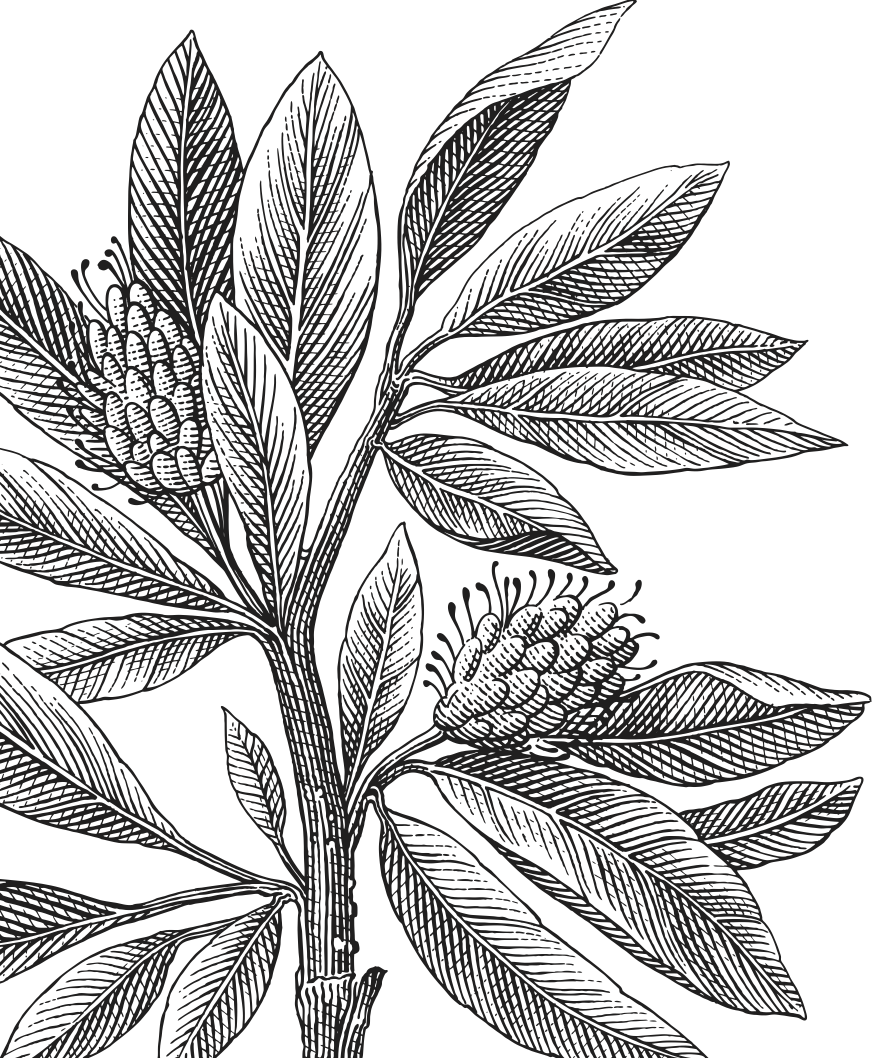
\includegraphics[keepaspectratio,scale=0.3]{img/lnu_etch.png} % Background picture
    }
}
\newcommand\BackgroundPicLogo{
    \put(30,740){
    
\includegraphics[keepaspectratio,scale=0.10]{img/logo.png} % Logo in upper left corner
    }
}

\title{	
\vspace{-8cm}
\begin{sidebar}
    \vspace{10cm}
    \normalfont \normalsize
    \Huge Report \\
    \vspace{-1.3cm}
\end{sidebar}
\vspace{3cm}
\begin{flushleft}
    \huge Project Course In Computer Science\\ 
    \it \LARGE - Analysis document
\end{flushleft}
\null
\vfill
\begin{textblock}{6}(10,13)
\begin{flushright}
\begin{minipage}{\textwidth}
\begin{flushleft} \large
\emph{Author:} Quasim Aljubarah, Michael Johansson, Tadas Lisauskas, Zeyuan Li, Robin Reijo and Robin Stempa\\ % Author
\emph{Supervisor:} Ola Petersson\\ % Supervisor
%\emph{Examiner:} Dr.~Mark \textsc{Brown}\\ % Examiner (course manager)
\emph{Semester:} VT 2016\\ % 
\emph{Subject:} 1DV508\\ % Subject area
\end{flushleft}
\end{minipage}
\end{flushright}
\end{textblock}
}

\date{} 

\begin{document}
\pagenumbering{gobble}
\newgeometry{left=5cm}
\AddToShipoutPicture*{\BackgroundPic}
\AddToShipoutPicture*{\BackgroundPicLogo}
\maketitle
\restoregeometry
\clearpage

\selectlanguage{english}

\tableofcontents

\newpage
\pagenumbering{gobble}
\pagenumbering{arabic}

%----------------------------------------------------------------------------------------
%
%	Here follows the actual text contents of the report.
%
%----------------------------------------------------------------------------------------

\section{Analysis}
This section will cover all the requirements for the webshop and define them.
\subsection{General requirements }
This table analyses the general requirements for the webshop.
\newline

\begin{table}[htbp]
	\centering
	\caption{My caption}
	\label{my-label}
	\begin{tabular}{|l|l|}
		\hline
		\textbf{ID}    & \textbf{Requirements}                                                                                                               \\ \hline
		\textbf{1}     & The webshop must contain any number of products.                                                                                    \\ \hline
		\textbf{1.1}   & All information about the products shall be stored in the database.                                                                 \\ \hline
		\textbf{1.1.1} & \begin{tabular}[c]{@{}l@{}}product must have:\\ -Product name\\ -Category\\ -Quantity\\ -Price\\ -Description\\ -Image\end{tabular} \\ \hline
		\textbf{1.1.2} & All products will be pre-defined to categories (Monitors,Computers, Etc.)                                                           \\ \hline
		\textbf{1.2}   & When an order is placed it must be added to the database                                                                            \\ \hline
		\textbf{1.2.1} & When an order is placed the quantity of the products must change                                                                    \\ \hline
	\end{tabular}
\end{table}
\subsection{Customer requirements}
This table will look into the customer requirements
\newline
\begin{table}[htbp]
	\centering
	\caption{My caption}
	\label{my-label}
	\begin{tabular}{|l|l|}
		\hline
		\textbf{ID}    & \textbf{Requirement}                                                                                                                                                                          \\ \hline
		\textbf{2}     & \begin{tabular}[c]{@{}l@{}}The customer must be able to browse the products in the following ways:\\ -Browse all products\\ -Search for a product\\ -Show products in a category\end{tabular} \\ \hline
		\textbf{2.1}   & It must be possible to click on a product to see more details about it.                                                                                                                       \\ \hline
		\textbf{2.2}   & The customer must be able to put a product in a cart.                                                                                                                                         \\ \hline
		\textbf{2.2.1} & The customer must be able to view the products in the cart.                                                                                                                                   \\ \hline
		\textbf{2.2.2} & The customer must be able to change the quantity of a product in the cart.                                                                                                                    \\ \hline
		\textbf{2.2.3} & \begin{tabular}[c]{@{}l@{}}The customer must be able to remove a product from the cart with one click with any \\ quantity.\end{tabular}                                                      \\ \hline
		\textbf{2.3}   & The customer must be able to place an order   .                                                                                                                                               \\ \hline
		\textbf{2.3.1} & \begin{tabular}[c]{@{}l@{}}When placing an order, a form must be shown where the customer enters his/her \\ contact details (email, address, phone number).\end{tabular}                      \\ \hline
		\textbf{2.3.2} & When an order is finalized the customer must receive an auto-generated order number.                                                                                                          \\ \hline
		\textbf{2.3.3} & The customer must be able to check the status of his/her order from the order number.                                                                                                         \\ \hline
	\end{tabular}
\end{table}
\subsection{Administrator requirements}
Last section will look into the requirements for the administrator view mode and the \mbox{functionalities} it must have.
\newline


\begin{table}[htpb]
	\centering
	\caption{Administrator requirements table}
	\label{my-label}
	\begin{tabular}{|l|l|}
		\hline
		\textbf{ID}    & \textbf{Requirement}                                                       \\ \hline
		\textbf{3}     & The webshop shall have an Admin system where an administrator can log on   \\ \hline
		\textbf{3.1}   & Administrator accounts and passwords shall be stored in the database.      \\ \hline
		\textbf{3.2}   & An administrator must be able to add a new product                         \\ \hline
		\textbf{3.2.1} & An administrator must be able to remove a product                          \\ \hline
		\textbf{3.2.2} & An administrator must be able to change information about a product        \\ \hline
		\textbf{3.2.3} & An administrator must be able to add a category                            \\ \hline
		\textbf{3.2.4} & An administrator must be able to remove a category                         \\ \hline
		\textbf{3.2.5} & An administrator must be able to change information about a category       \\ \hline
		\textbf{3.3}   & An administrator must be able to add a new administrator account           \\ \hline
		\textbf{3.3.1} & An administrator must be able to remove a administrator account            \\ \hline
		\textbf{3.4}   & An administrator must be able to view all orders                           \\ \hline
		\textbf{3.4.1} & An administrator must be able update the order status on every order       \\ \hline
		\textbf{3.4.2} & The order status can only be New, Shipped, Delayed, Delivered and Returned \\ \hline
	\end{tabular}
\end{table}

\end{document}
